\thispagestyle{empty}

\section*{Abstract}
\label{sec:abstract}

Text Summarization can be a powerful tool to reduce the amount of time for reading documents, articles or even research papers. The thesis is divided into a larger state of the art part and a shorter prototype part. The state of the art part examines the concepts of text generation and text summarization with the focus on my prototype. Most concepts are introduced in order to fully understand how my prototype is able to achieve the text generation, except for some advanced thinking outside the box concepts, which cannot be applied by me, because it would exceed this thesis. My prototype is trained on the Amazon-fine-food-reviews from \textit{www.kaggle.com} and the results are evaluated on the Rouge and BLEU scores. In the end, I further introduce some performance enhancements. 

\null\newpage

\section*{Acknowledgement}

I would like to thank Professor Dr. Albrecht Holl for supervising my Bachelor Thesis. He always supported me and helped me a lot when I was facing problems regarding my thesis. \\ \\ \\ \\

\begin{center}
\LARGE{\textit{I dedicate my thesis to Wong Chui Shan} 
\begin{CJK*}{UTF8}{bsmi} 
	(黃翠珊)
\end{CJK*}
}
\end{center}
\null\newpage

\section*{Preface I}
\label{sec:prolog_1}

The following thesis was created during the seventh and last semester at the Georg Simon Ohm University of Applied Science. 
Within the last three semesters, I realized that my primary interest among all IT related topics is artificial intelligence.

My interest started basically with a group IT-project, in which my team and I programmed an autonomously driving remote control car with a deep neural network together with a Raspberry Pi 3B+. From this first project on, I selected all my further elective courses to be related to machine learning or data science in any possible way. I wanted to increase my knowledge further, so I searched for a website that provides courses related to AI. I found \textit{www.udacity.com}, which offers courses in cooperation with top IT companies, such as Google, Airbnb, or Microsoft. Out of curiosity, I bought the course \textit{Natural Language Processing}. After successfully finishing it, I was encouraged to write my bachelor thesis in a \textit{Natural Language Processing} related topic. 
Together with my professor \textit{Prof. Dr. Alfred Holl}, I worked out a structured methodological table for the entire structure of this paper. 
Even though Natural Language Processing is just a subfield of machine learning, the current state-of-the-art research is far beyond what I can research within a bachelor thesis. I decided to write my thesis about the subfield \textit{text summarization} within NLP. I research about the history of text summarization systems and the current state of the art.
Further I program a prototype in python to apply this knowledge.
\null\newpage

\section*{Preface II}
\label{sec:prolog_2}
For my research, I encountered a lot of old and recently published papers, mostly from \textit{https://arxiv.org/}. 
Reading through the papers requires much prior knowledge, especially in mathematics, which I learned during my semester in Hong Kong at the City University of Hong Kong. 
Machine Learning and, more specifically, NLP is not an intuitive study. All of my explanations could be presented with their mathematical notations as well, but it would exceed this thesis by far if I would explain every technological change based on its maths. I rather want to give a detailed overview and if the reader is encouraged to learn more about it, he/she knows then the keywords to search for it and all of the papers are cited as well.
During the five-month development process of the bachelor thesis, I gained much knowledge. I recognized that NLP is a vast topic, always under research. To keep up to date with the latest publications requires much effort. \\
To give a full state-of-the-art review about \textit{all} text generation related disciplines is not possible within this thesis. For that reason, I have primarily focused on text summarization part.


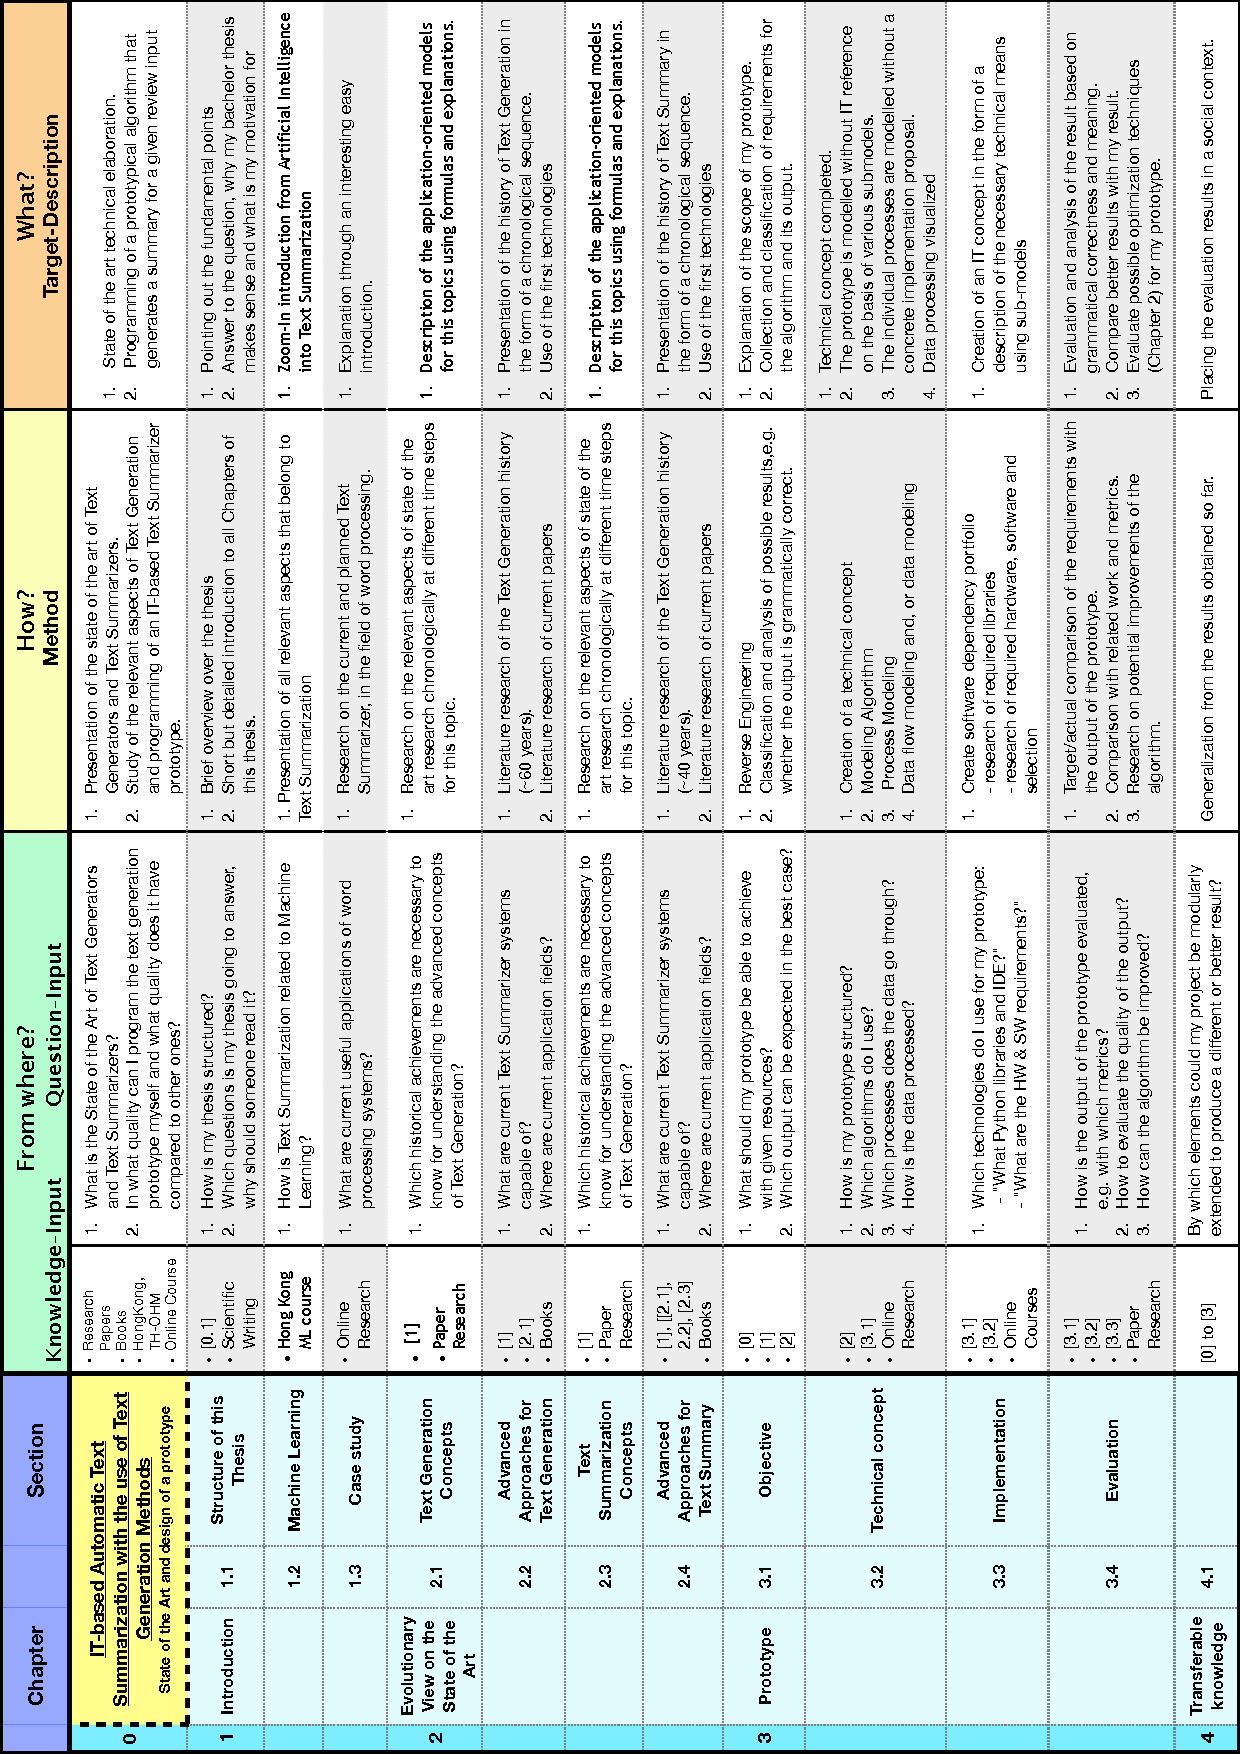
\includepdf[fitpaper=true, pages=-]{methoden_matrix.pdf}

